\Chapter{Software}\label{chapter:softwareChapter}

\Section[Introduction]{Introduction}\label{sec:swIntroductionSection}\\

Providing just a hardware solution is unacceptable for adoption, a software package that is easy to use and extensible is a necessary feature. Long are the days of the average VR graphics programmer using OpenGL to create simple prototypes. Game engines dominate the interactive media industry and VR SDKs were quick to target them.

\noindent\textbf{The Choice of the Unity3D Game Engine}
\begin{center}
	\textcolor{OliveGreen}{Purpose: Explain why we chose the Unity Game Engine}
	
	\begin{table}[H]
		\centering
		\renewcommand\arraystretch{0.5}
		\begin{tabular}{|l|}
			\hline 
			Topics To Write About \\ 
			\hline 
			Usage of Game Engines \\
			2nd wave VR in game engines  \\
			Unity vs Unreal \\  
			easy development in programming \\ 
			explain the role of display cameras \\ 
			goal for programming the vden  \\
			\hline 
		\end{tabular}
	\end{table}
\end{center}


\begin{figure}[H]
	\centering
	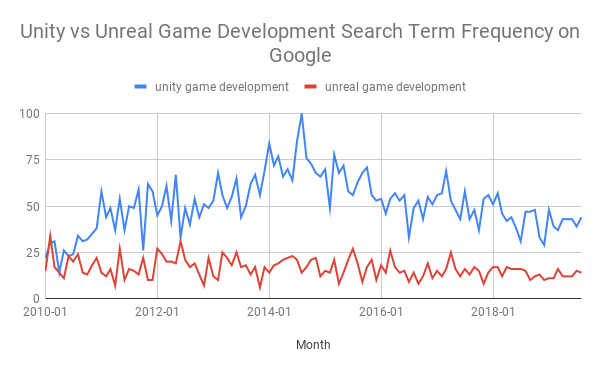
\includegraphics[width=6in]{images/googletrends-unity-game-dev-vs-unreal}
	\caption[Unity vs Unreal Search Term Frequency]{A graph from Google Trends showing the search term frequency of "unity game development" versus "unreal game engine development" from 2010 (Marking the release of version 3 of Unity). The vertical axis represents the percentage of popularity.}
	\label{fig:googletrends-unity-game-dev-vs-unreal}
\end{figure}

\filbreak
Unity3D is a game engine for creating interactive media. Launched in 2005, the goal was to create an affordable system for amateur game developers.\cite{unityHistory} By focusing on a simple asset pipeline and workflow, Unity3D thrived and by 2010 had over 200,000 registered users. Quickly, Unity became the \#1 platform for game development. \cite{unity3ReleaseNews}

The major competition to Unity3D is the Unreal Engine. Initially developed by Tim Sweeney, this engine was designed to push the limits of graphics and realism. Not only has it received a 2014 Guinness World Record for "Most Successful Game Engine", but also a long list from game developers and film productions alike.\cite{unrealAwards} However as shown in Figure \ref{fig:googletrends-unity-game-dev-vs-unreal}, Unity3D is more searched on Google for game development topics supporting the notion that it is the preferred tool for most games. 

A Bachelor's thesis written by Simo Ahola describes the steps necessary to build a Virtual Reality application in the Unity3D game engine supporting two different headsets: the HTC Vive and Oculus GO. By just downloading the individual SDKs then dragging and dropping the associated prefabricated component, Simo had easily developed a VR application.\cite{aholaUnityVR} 

It is of my personal desire to make CAVE development as simple and accessible as a headset. Unity's history of simplicity has positioned it in the forefront of VR development, making it the preferred platform for the vDen. 


\filbreak
\Section[Unity SDK]{Unity SDK}\label{sec:unitySDKSection} \\
\begin{center}
	\textcolor{OliveGreen}{Purpose: Explain the design of the SDK}
	
	\begin{table}[H]
		\centering
		\renewcommand\arraystretch{0.5}
		\begin{tabular}{|l|}
			\hline 
			Topics To Write About \\ 
			\hline 
			structure of vive sdk \\
			describe how easy the vive is  \\
			emulate the structure of vive \\  
			explain the role of eye cameras \\ 
			explain the role of display cameras \\ 
			how did we implement head tracking  \\
			SDK configuration  \\
			\hline 
		\end{tabular}
	\end{table}
\end{center}

The simple act of downloading an SDK and dragging the necessary components into your scene sounds so fundamental, however it was not until WYSIWYG game engines became popular for this to happen. The architecture of the vDen SDK revolves around this concept.

To guide development, we defined three goals for our system: rendering immediately upon importing, allowing full extension and of peripherals, and lastly simulating the vDen rendering in Unity itself.

The core rendering system govern the functionality of the eye and display cameras.

\noindent\textbf{Eye Cameras} \\
\begin{center}
	\textcolor{OliveGreen}{
		Purpose: Explain the how the eye cameras work
	}
	
	\begin{table}[H]
		\centering
		\renewcommand\arraystretch{0.5}
		\begin{tabular}{|l|}
			\hline 
			Topics To Write About \\ 
			\hline 
			Purpose \\
			Frustum Calculation \\
			\hline 
		\end{tabular}
	\end{table}
\end{center}

\begin{figure}[H]
	\centering
	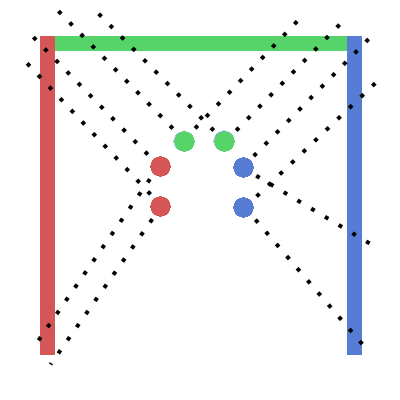
\includegraphics[width=3in]{images/camera-pairs}
	\caption[The Pairing of Eye Cameras]{The Eye Cameras are paired together and are related to a specific screen. Each camera pair has space in-between related to the inter-pupillary distance of the user's head. The floor cameras are missing in the graphic, but are in the SDK, bringing the total to 8 eye cameras.}
	\label{fig:eye-camera-pairing}
\end{figure}

Eye cameras capture an image that represents the view from a user's physical eye. As shown in Figure \ref{fig:eye-camera-pairing}, there are two cameras per screen, totaling 8 in the SDK. A pair of cameras are spaced apart along the shared axis with the distance equivalent to the user's interpupillary distance. Futhermore, each pair needs to remain orthogonal to the others. Lastly, because the screens represent a window to the world, we need to calculate a custom frustum for each camera.

\begin{figure}[H]
	\centering
	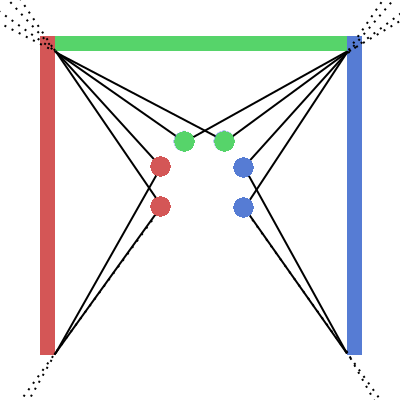
\includegraphics[width=3in]{images/camera-pairs-calibrated}
	\caption[The New Frustum of Eye Cameras]{Shows the new frustum of each camera after calculation. This provides the correct view as our physical screens represent windows into the world}
	\label{fig:eye-camera-frustum}
\end{figure}

Looking at the differences between Figure \ref{fig:eye-camera-pairing} and Figure \ref{fig:eye-camera-frustum}, we can immediately see the frustum is bounded to the the screen. This bounding guarantees that nothing is rendered outside of the screens. 

--- FIXME ---
The calcuation of a new frustum is easy. We need to determine the

\filbreak
\noindent\textbf{Display Cameras} \\
\begin{center}
	\textcolor{OliveGreen} {
		Purpose: Explain the display cameras
	}
	
	\begin{table}[H]
		\centering
		\renewcommand\arraystretch{0.5}
		\begin{tabular}{|l|}
			\hline 
			Topics To Write About \\ 
			\hline 
			Purpose \\
			Merging images together \\
			\hline 
		\end{tabular}
	\end{table}
\end{center}

Display Cameras will output the final image for the projectors. With one camera per projector, the vDen has four total. The camera is associated with a pair of eye cameras and is responsible for merging their output together, left-right or top-bottom, for sterescopy, then rendering on the calibration mesh.


\filbreak
\noindent\textbf{Head Tracking} \\
\begin{center}
	\textcolor{OliveGreen} {
		Purpose: Explain the head tracking system
	}
	
	\begin{table}[H]
		\centering
		\renewcommand\arraystretch{0.5}
		\begin{tabular}{|l|}
			\hline 
			Topics To Write About \\ 
			\hline 
			Purpose \\
			Utilizing the SteamVR trackable object \\
			Sync virtual and physical positions \\
			\hline 
		\end{tabular}
	\end{table}
\end{center}

A core feature of Virtual Reality is the generation of perspective correct imagery. This is done by understanding the head position and how the eyes view the scene. In order to track the head, the user dons a trackable baseball cap the tracking system syncs its position with the collection of eye cameras.


\filbreak
\Section[Calibrator]{Calibrator}\label{sec:CalibratorSection} \\
\begin{center}
	\textcolor{OliveGreen}{
		Purpose: Explain the design of the Calibrator
	}
	
	\begin{table}[H]
		\centering
		\renewcommand\arraystretch{0.5}
		\begin{tabular}{|l|}
			\hline 
			Topics To Write About \\ 
			\hline 
			Dragging each corner to fill the surface \\
			Checking corner image alignment \\
			Checking uniform scaling \\
			User Interaction \\
			Per Project JSON File\\
			\hline 
		\end{tabular}
	\end{table}
\end{center}

\Section[Dashboard]{Dashboard}\label{sec:dashboardSection} \\
\begin{center}
	\textcolor{OliveGreen}{
		Purpose: Explain the design of the dashboard
	}
	
	\begin{table}[H]
		\centering
		\renewcommand\arraystretch{0.5}
		\begin{tabular}{|l|}
			\hline 
			Topics To Write About \\ 
			\hline 
			Purpose \\
			Development \\
			Project Management \\
			Config Management \\
			Projector Control \\
			\hline 
		\end{tabular}
	\end{table}
\end{center}

\clearpage
